% Appendix Template

\chapter{Critical Concentrations} % Main appendix title

\label{Appendix_CriticalConcentrations} % Change X to a consecutive letter; for referencing this appendix elsewhere, use \ref{AppendixX}

\begin{figure}[!th]
\centering
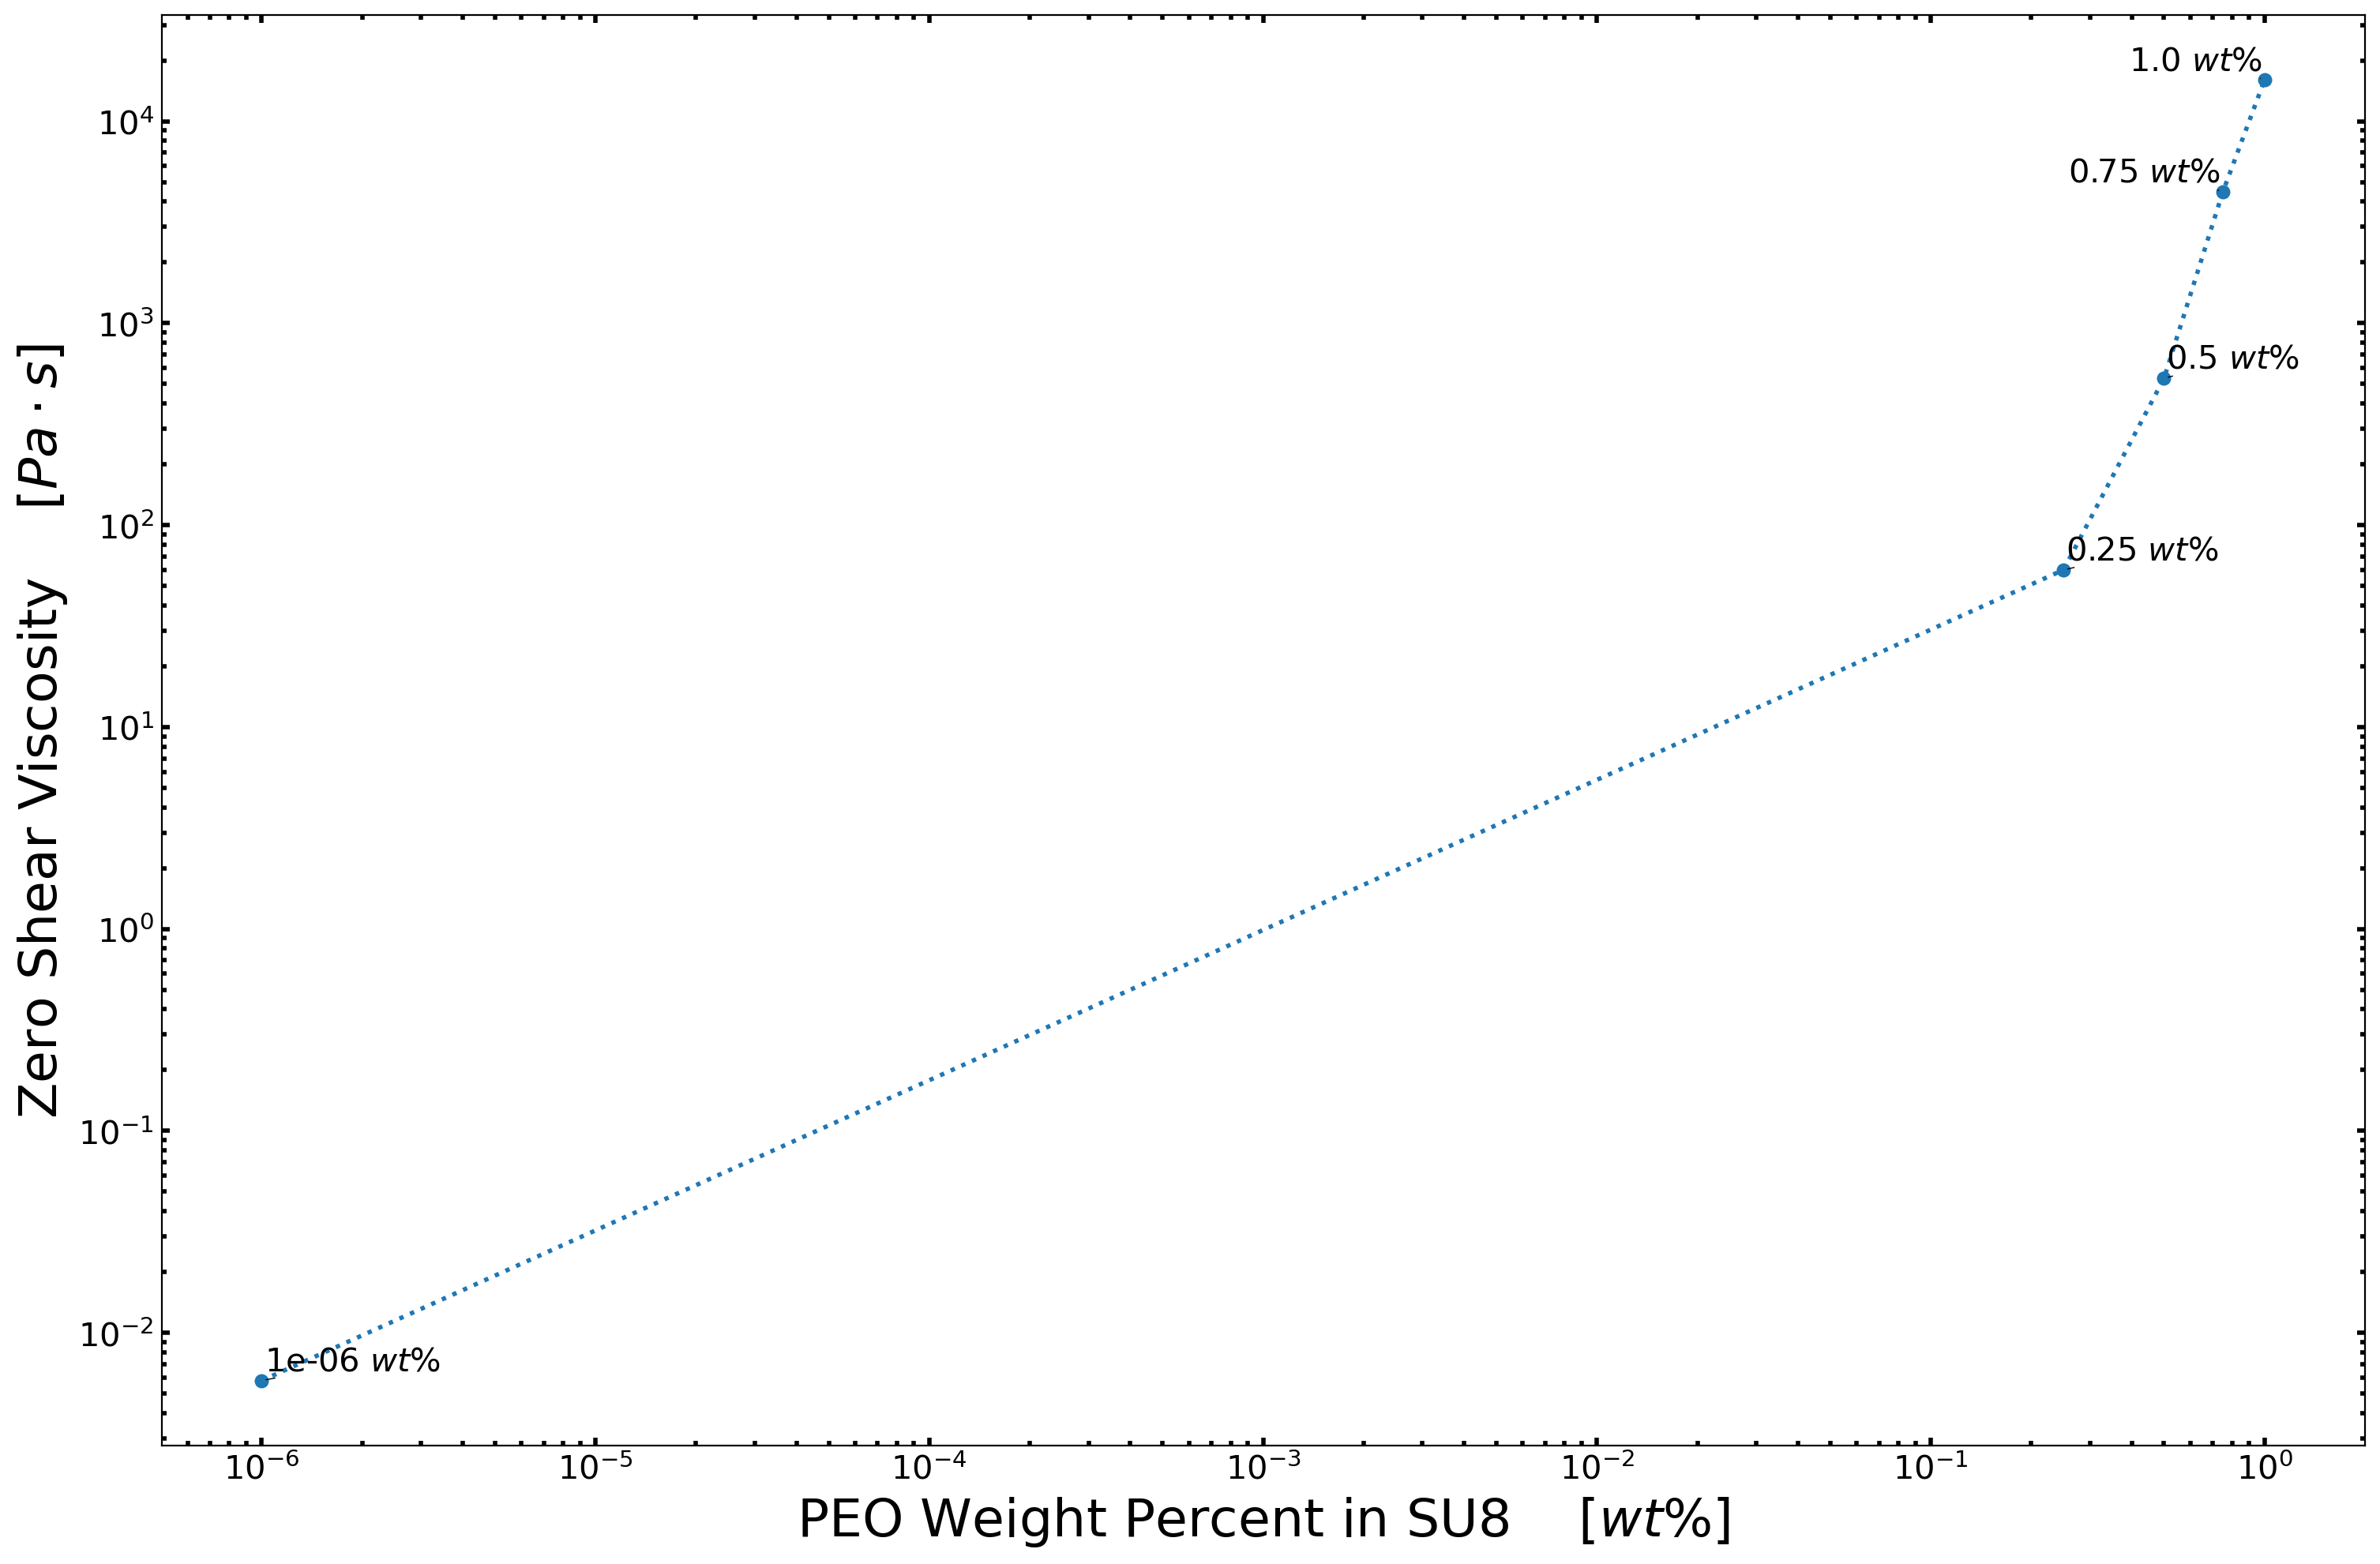
\includegraphics[width=\textwidth]{./Figures/c_vs_v_PEOinSU8.png}
\decoRule
\caption[Viscosity as a function of shear rate for Poly(Ethylene Oxide) (PEO) and SU-8 2002 solutions]{Viscosity as a function of shear rate for Poly(Ethylene Oxide) (PEO) and SU-8 2002 solutions}
\label{fig:c_vs_v_PEOinSU8}
\end{figure}

\begin{figure}[!th]
\centering
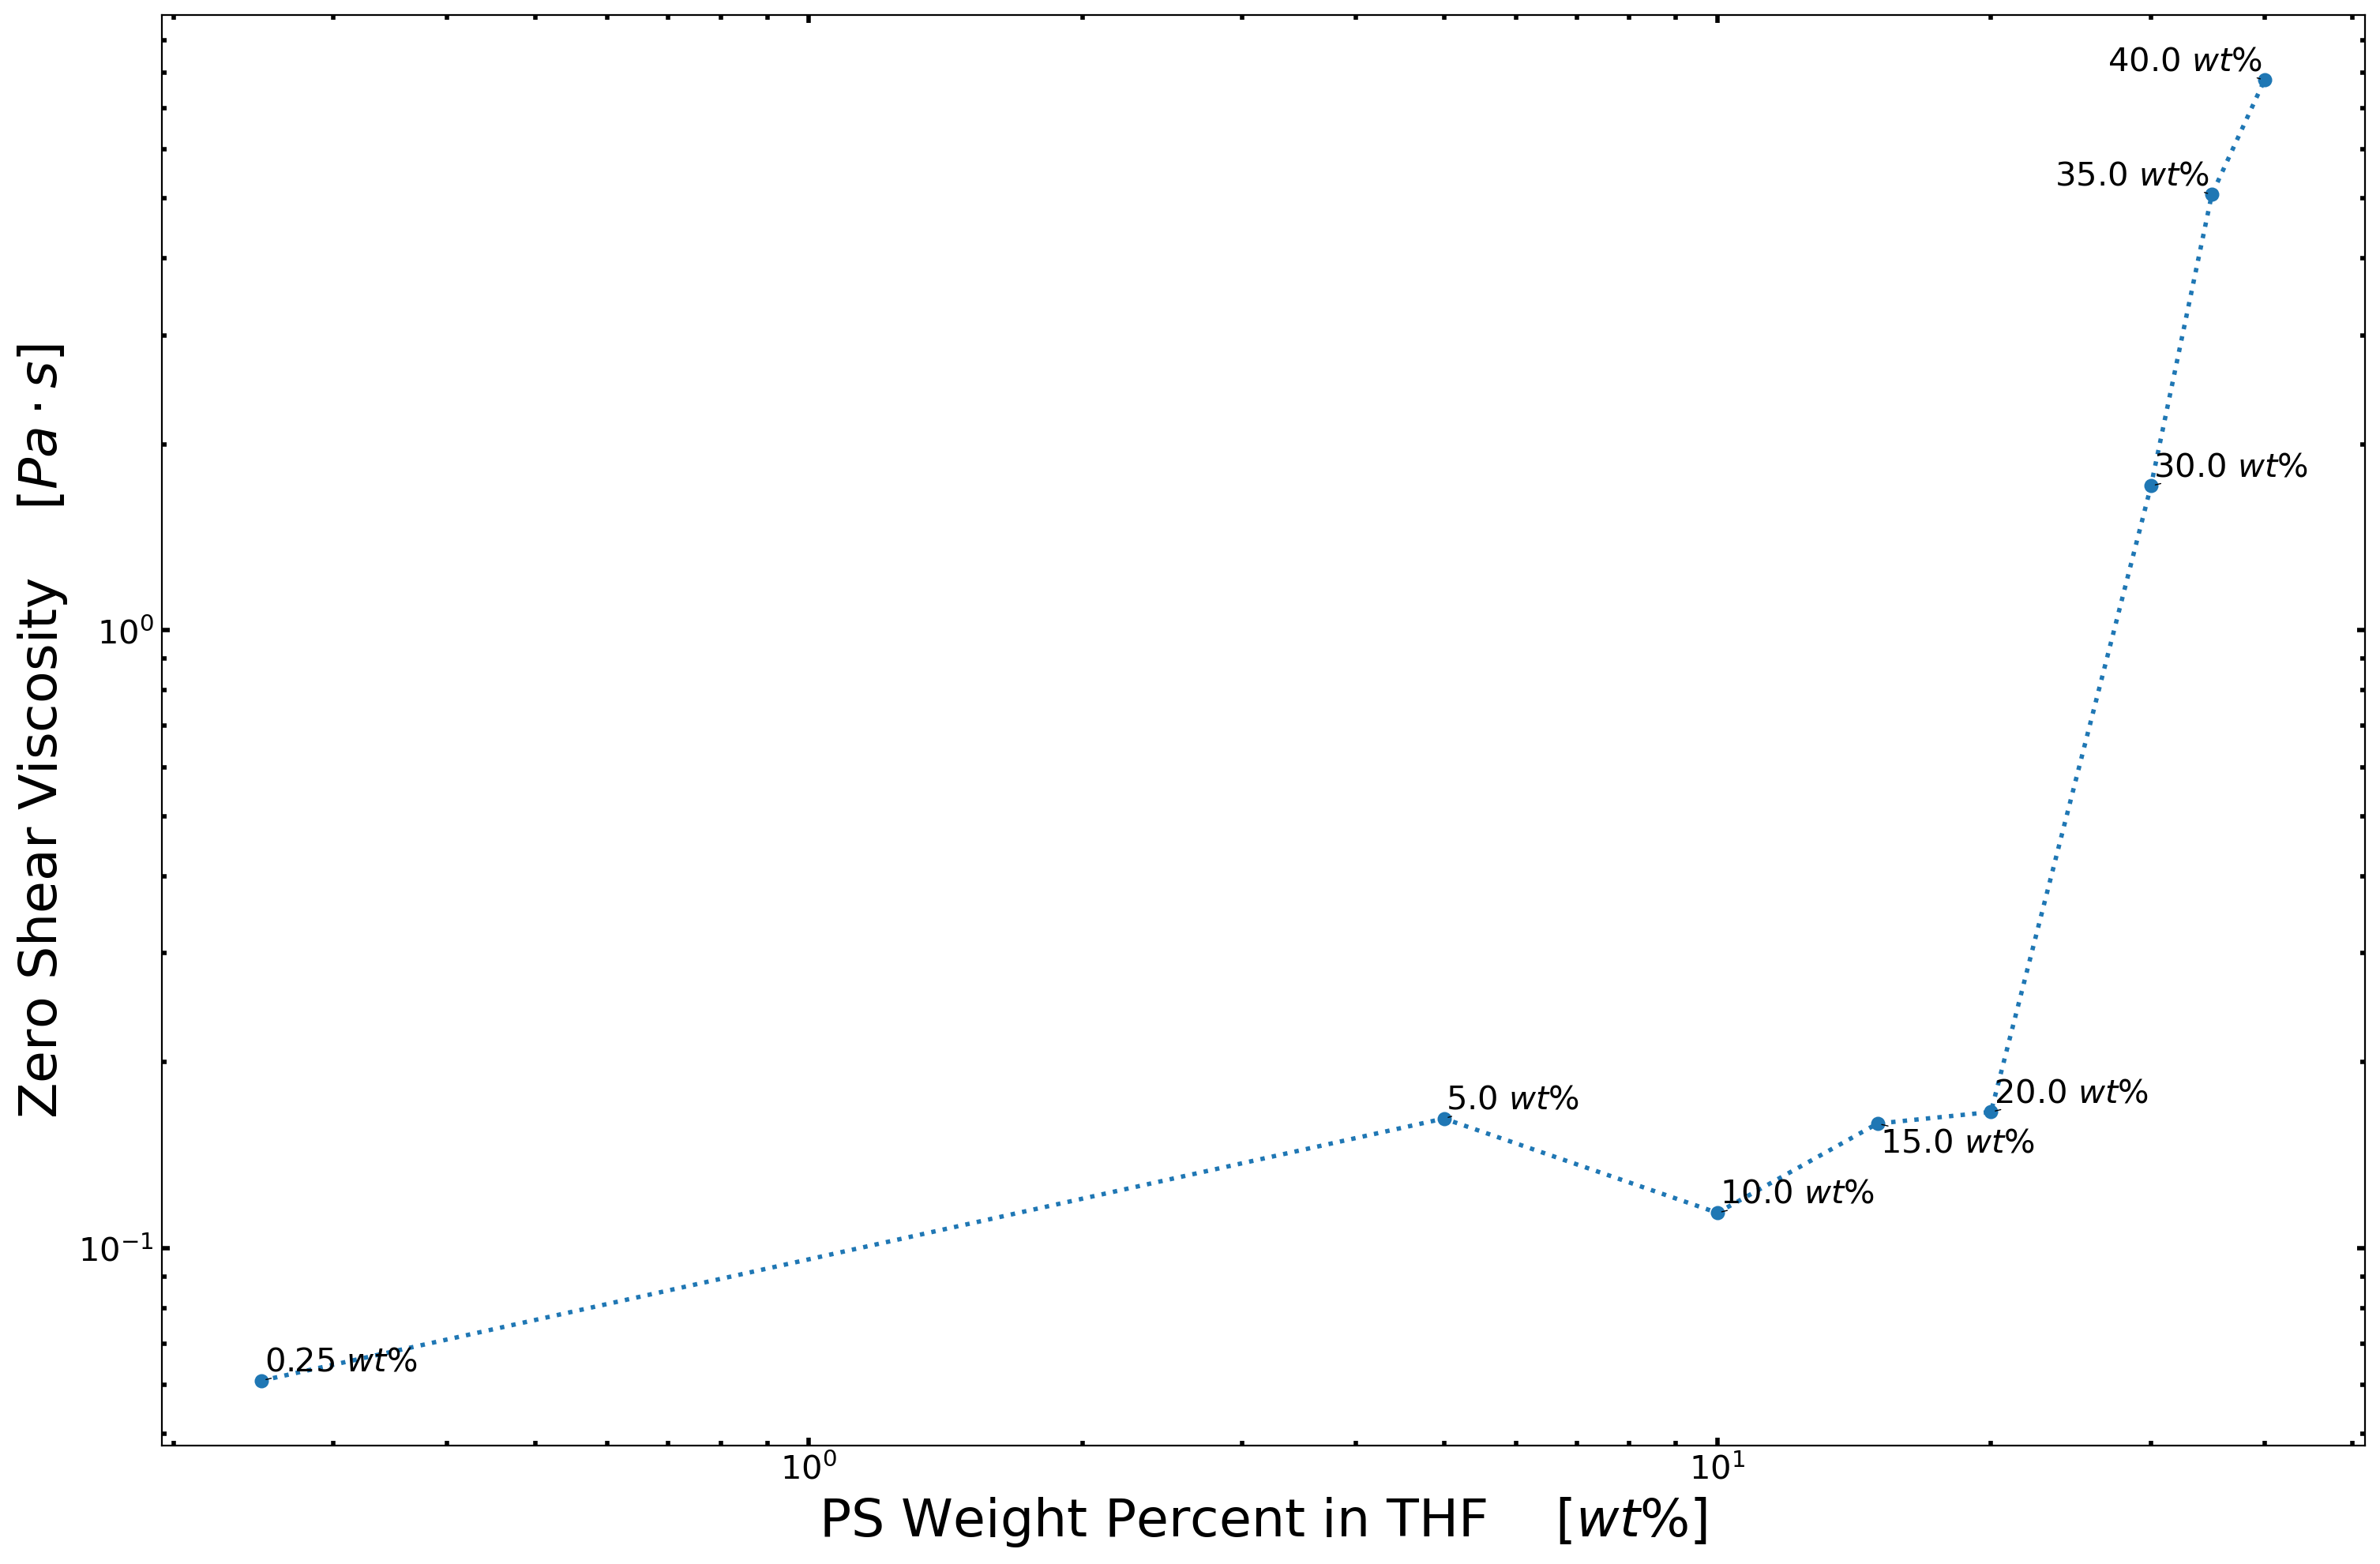
\includegraphics[width=\textwidth]{./Figures/c_vs_v_PSinTHF.png}
\decoRule
\caption[Viscosity as a function of shear rate for Polystyrene (PS) and Tetrahydrofuran (THF) solutions]{Viscosity as a function of shear rate for Polystyrene (PS) and Tetrahydrofuran (THF) solutions}
\label{fig:c_vs_v_PSinTHF}
\end{figure}

\begin{figure}[!th]
\centering
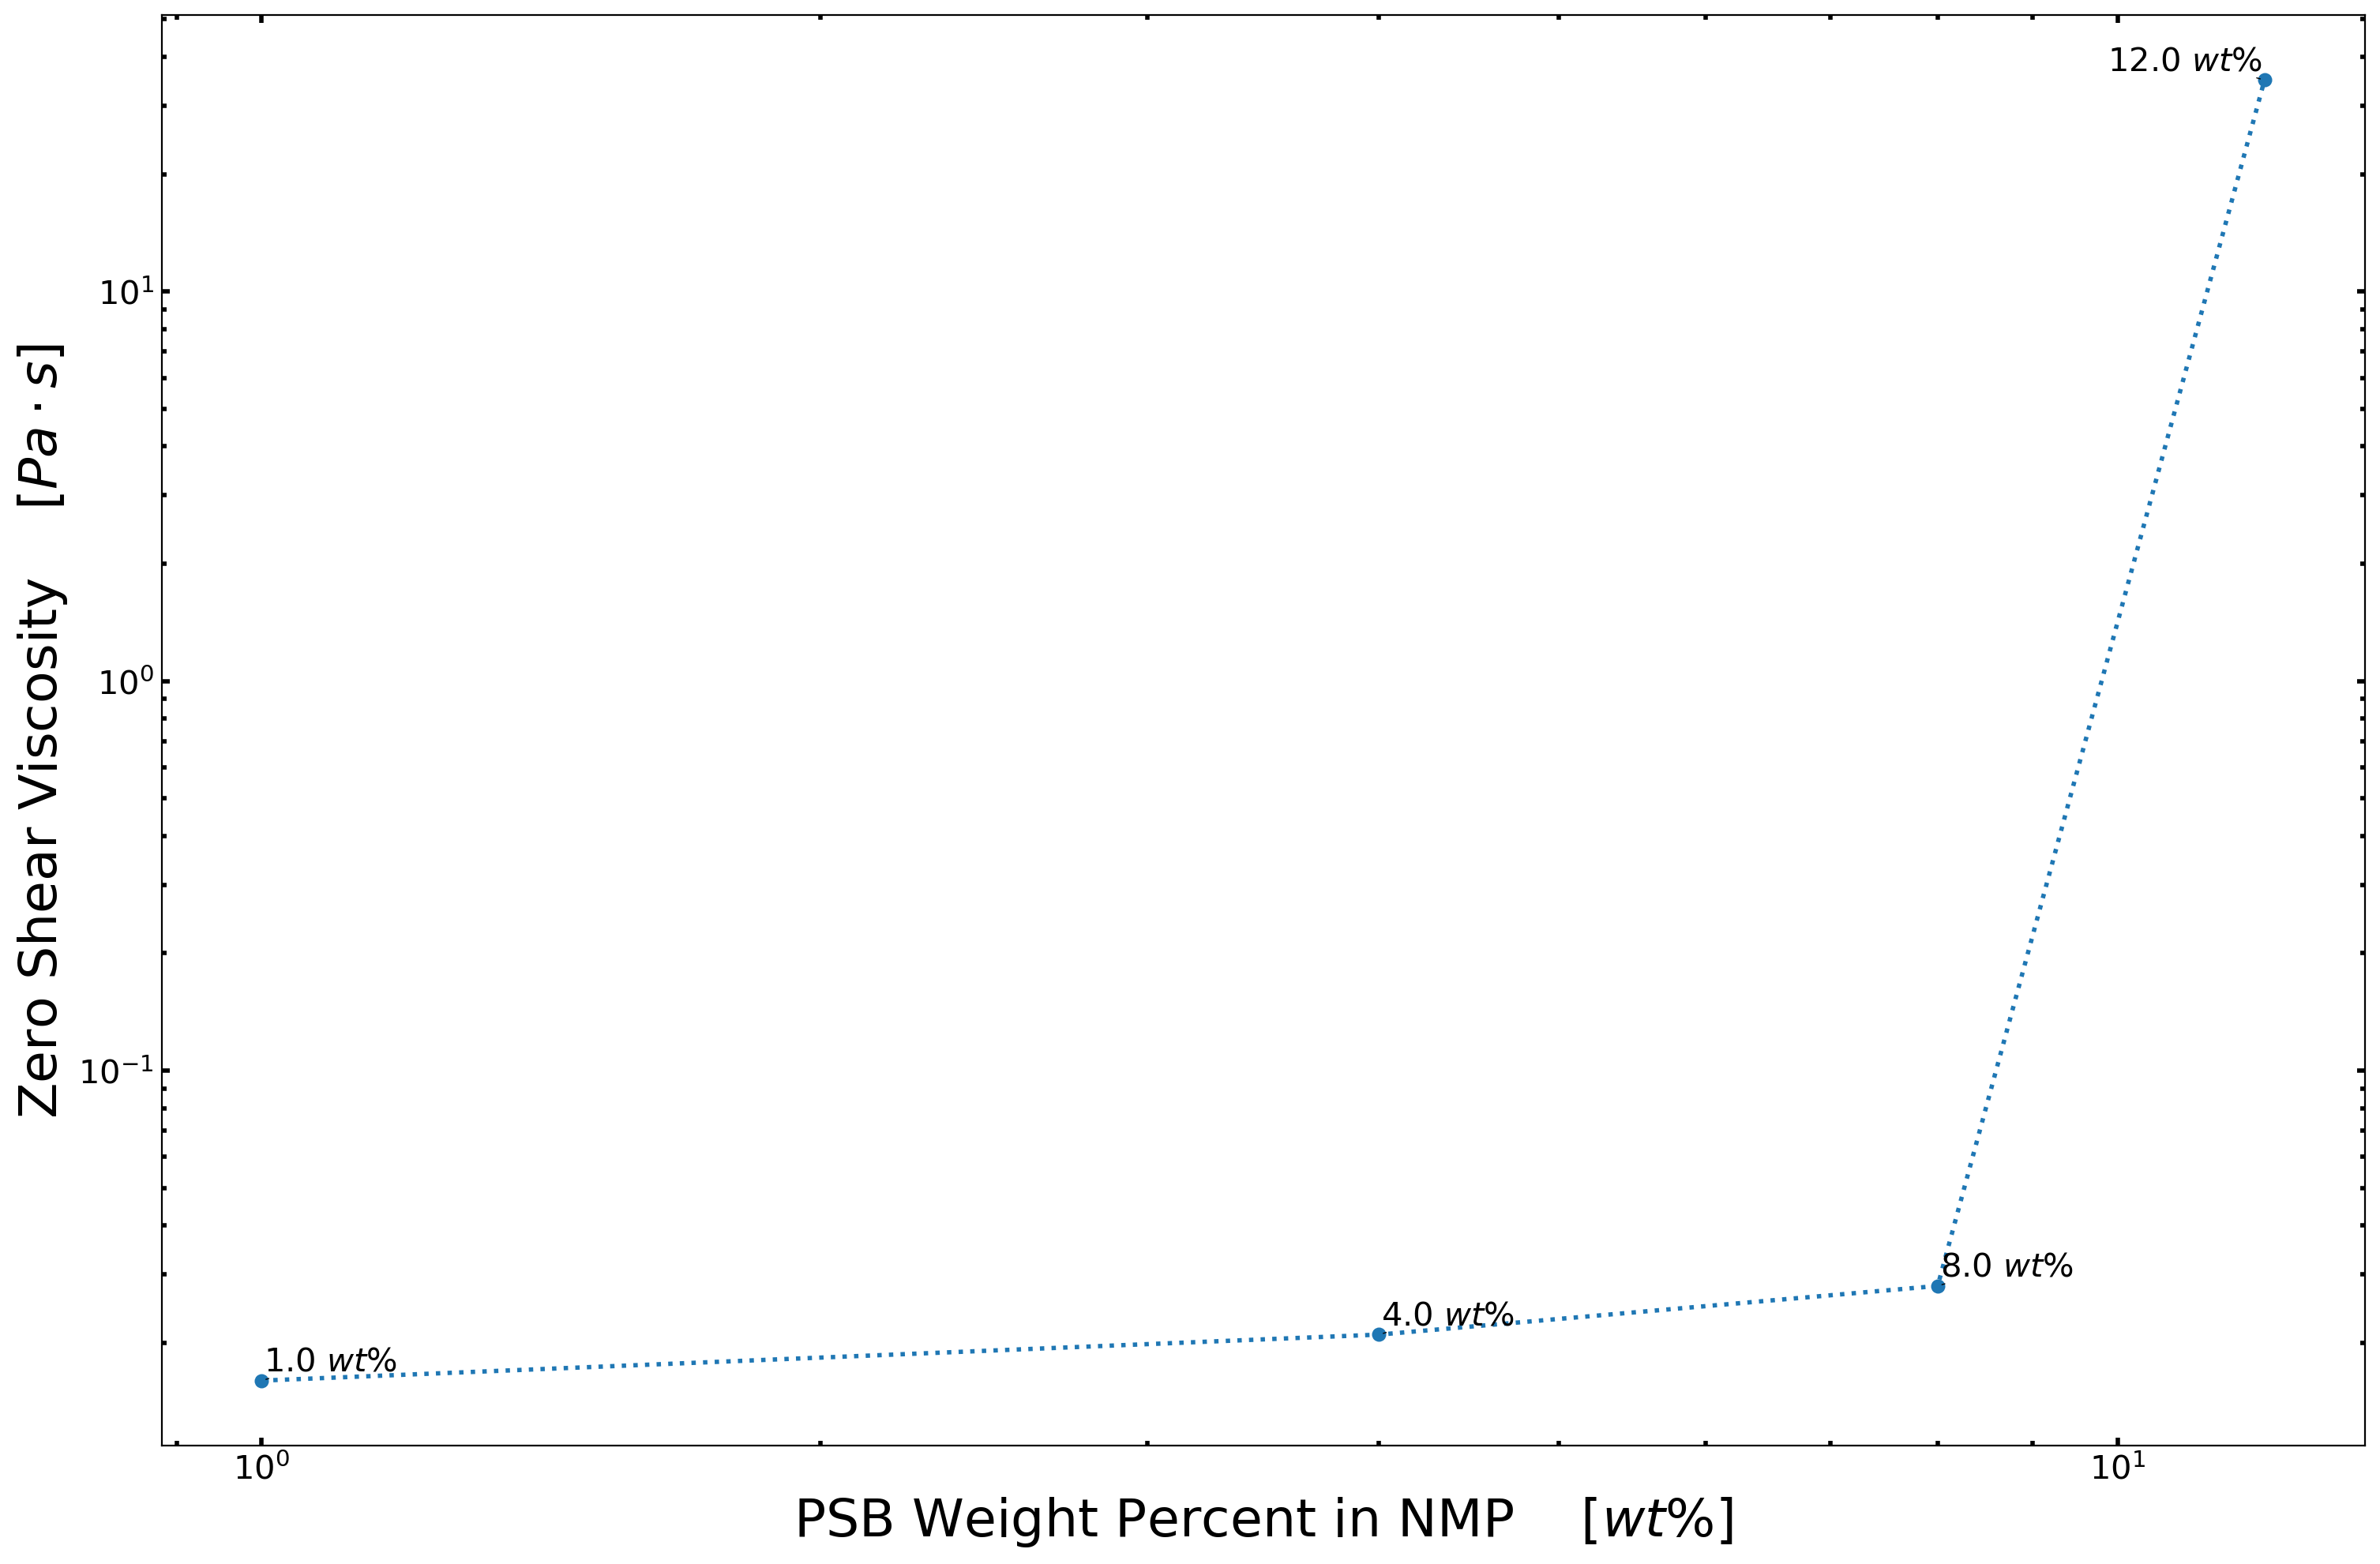
\includegraphics[width=\textwidth]{./Figures/c_vs_v_PSBinNMP.png}
\decoRule
\caption[Viscosity as a function of shear rate for Poly(Styrene-co-Butadiene) (PSB) and 1-Methyl-2-Pyrrolidinone (NMP) solutions]{Viscosity as a function of shear rate for Poly(Styrene-co-Butadiene) (PSB) and 1-Methyl-2-Pyrrolidinone (NMP)}
\label{fig:c_vs_v_PSBinNMP}
\end{figure}

\begin{figure}[!th]
\centering
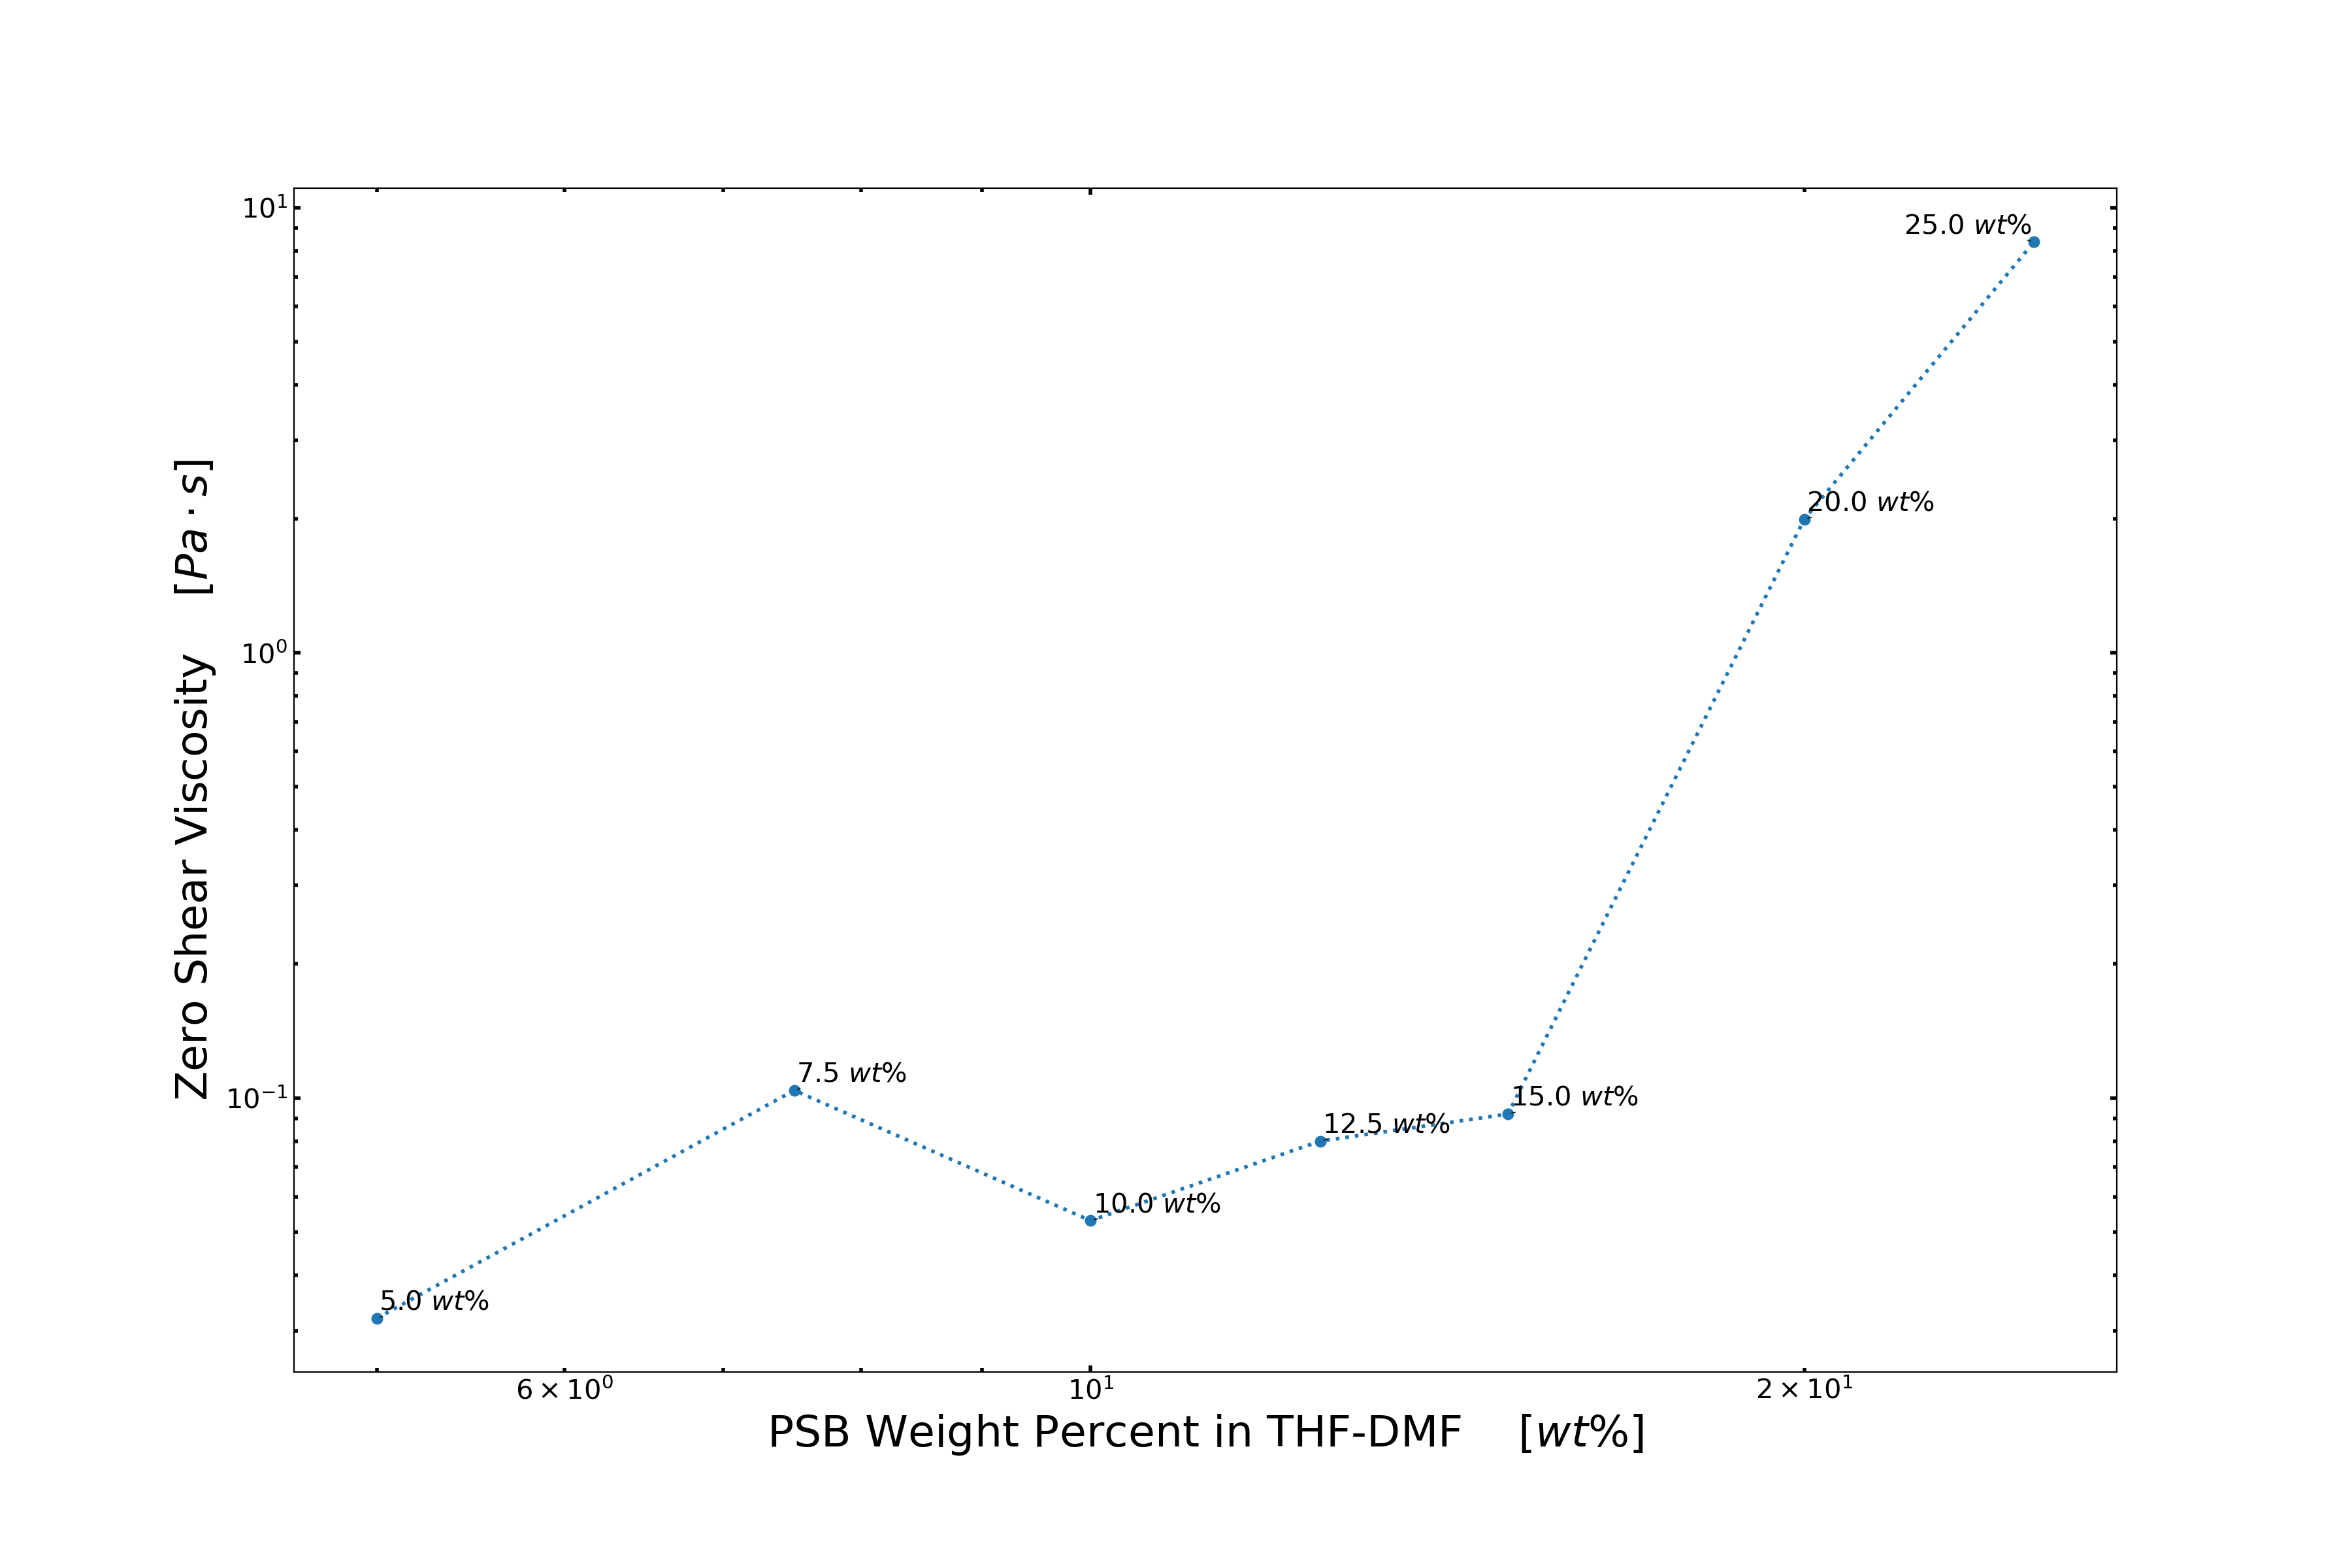
\includegraphics[width=\textwidth]{./Figures/c_vs_v_PSBinTHF-DMF.png}
\decoRule
\caption[Viscosity as a function of shear rate for Poly(Styrene-co-Butadiene) (PSB), Tetrahydrofuran (THF) and N,N-Dimethylformamide (DMF) solutions]{Viscosity as a function of shear rate for Poly(Styrene-co-Butadiene) (PSB), Tetrahydrofuran (THF) and N,N-Dimethylformamide (DMF) solutions}
\label{fig:c_vs_v_PSBinTHF-DMF}
\end{figure}

\begin{figure}[!th]
\centering
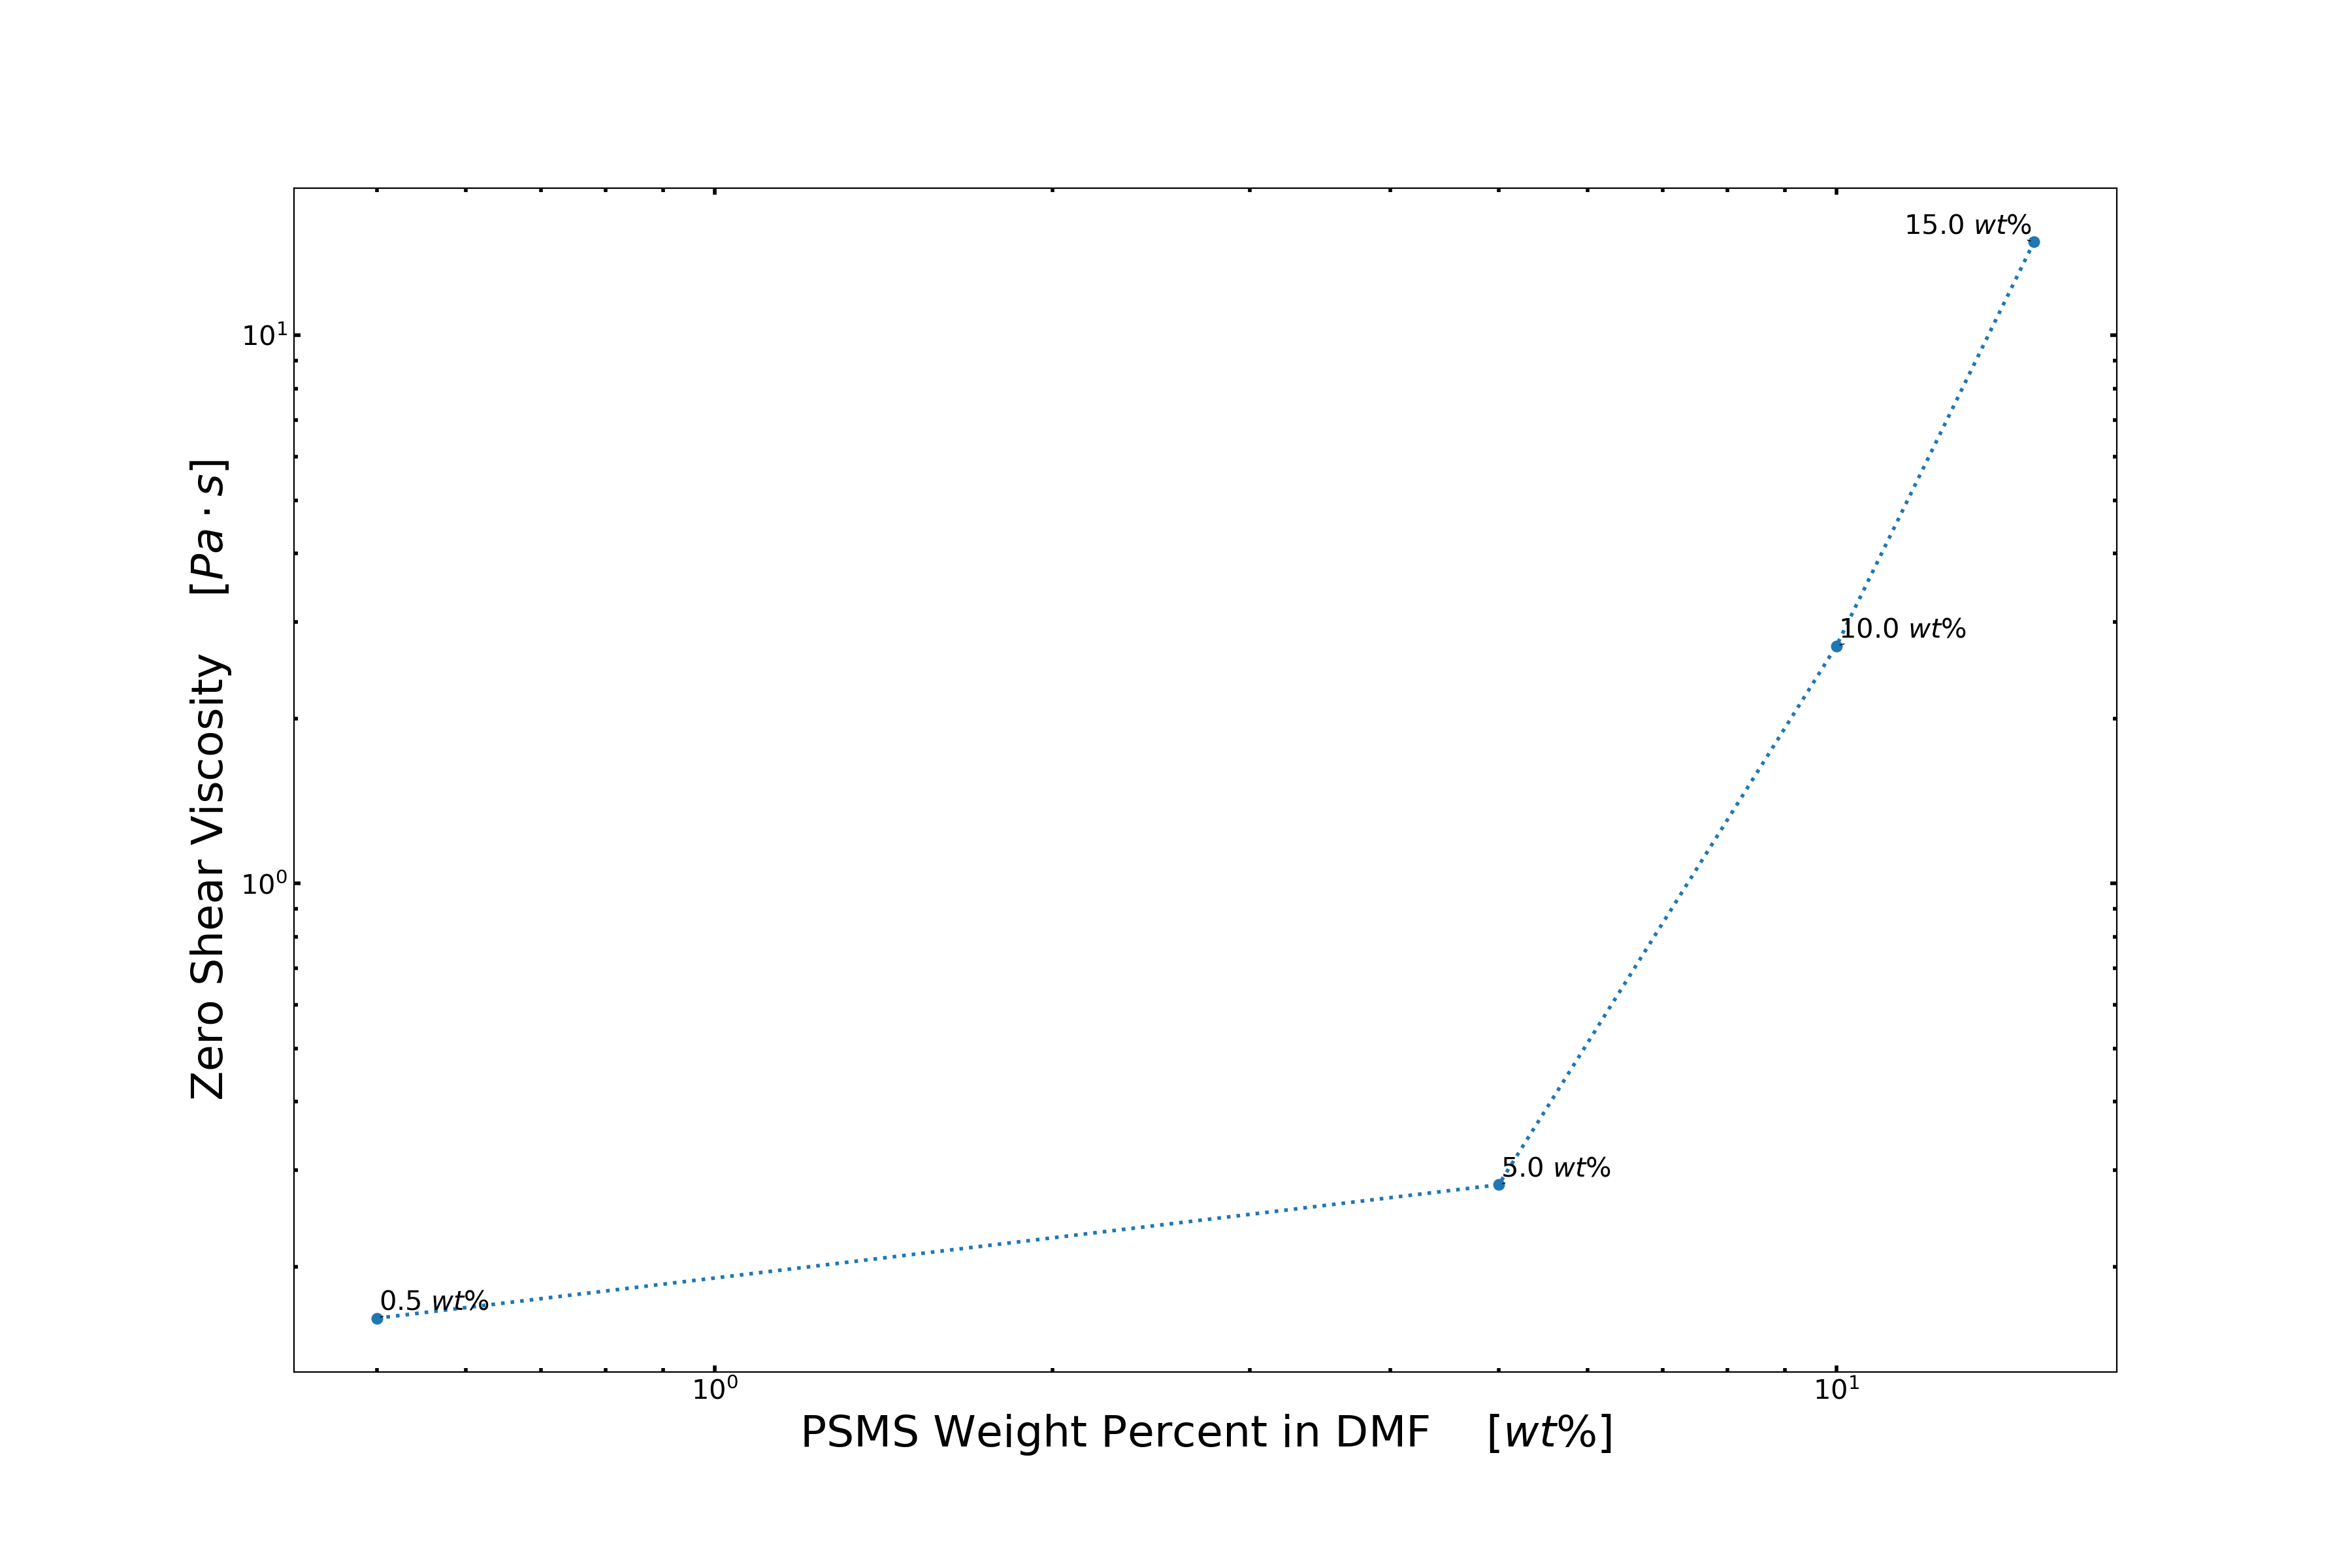
\includegraphics[width=\textwidth]{./Figures/c_vs_v_PSMSinDMF.png}
\decoRule
\caption[Viscosity as a function of shear rate for Poly(Styrene-co-alpha-Methylstyrene) (PSMS) and N,N-Dimethylformamide (DMF) solutions]{Viscosity as a function of shear rate for Poly(Styrene-co-alpha-Methylstyrene) (PSMS) and N,N-Dimethylformamide (DMF) solutions}
\label{fig:c_vs_v_PSMSinDMF}
\end{figure}

\begin{figure}[!th]
\centering
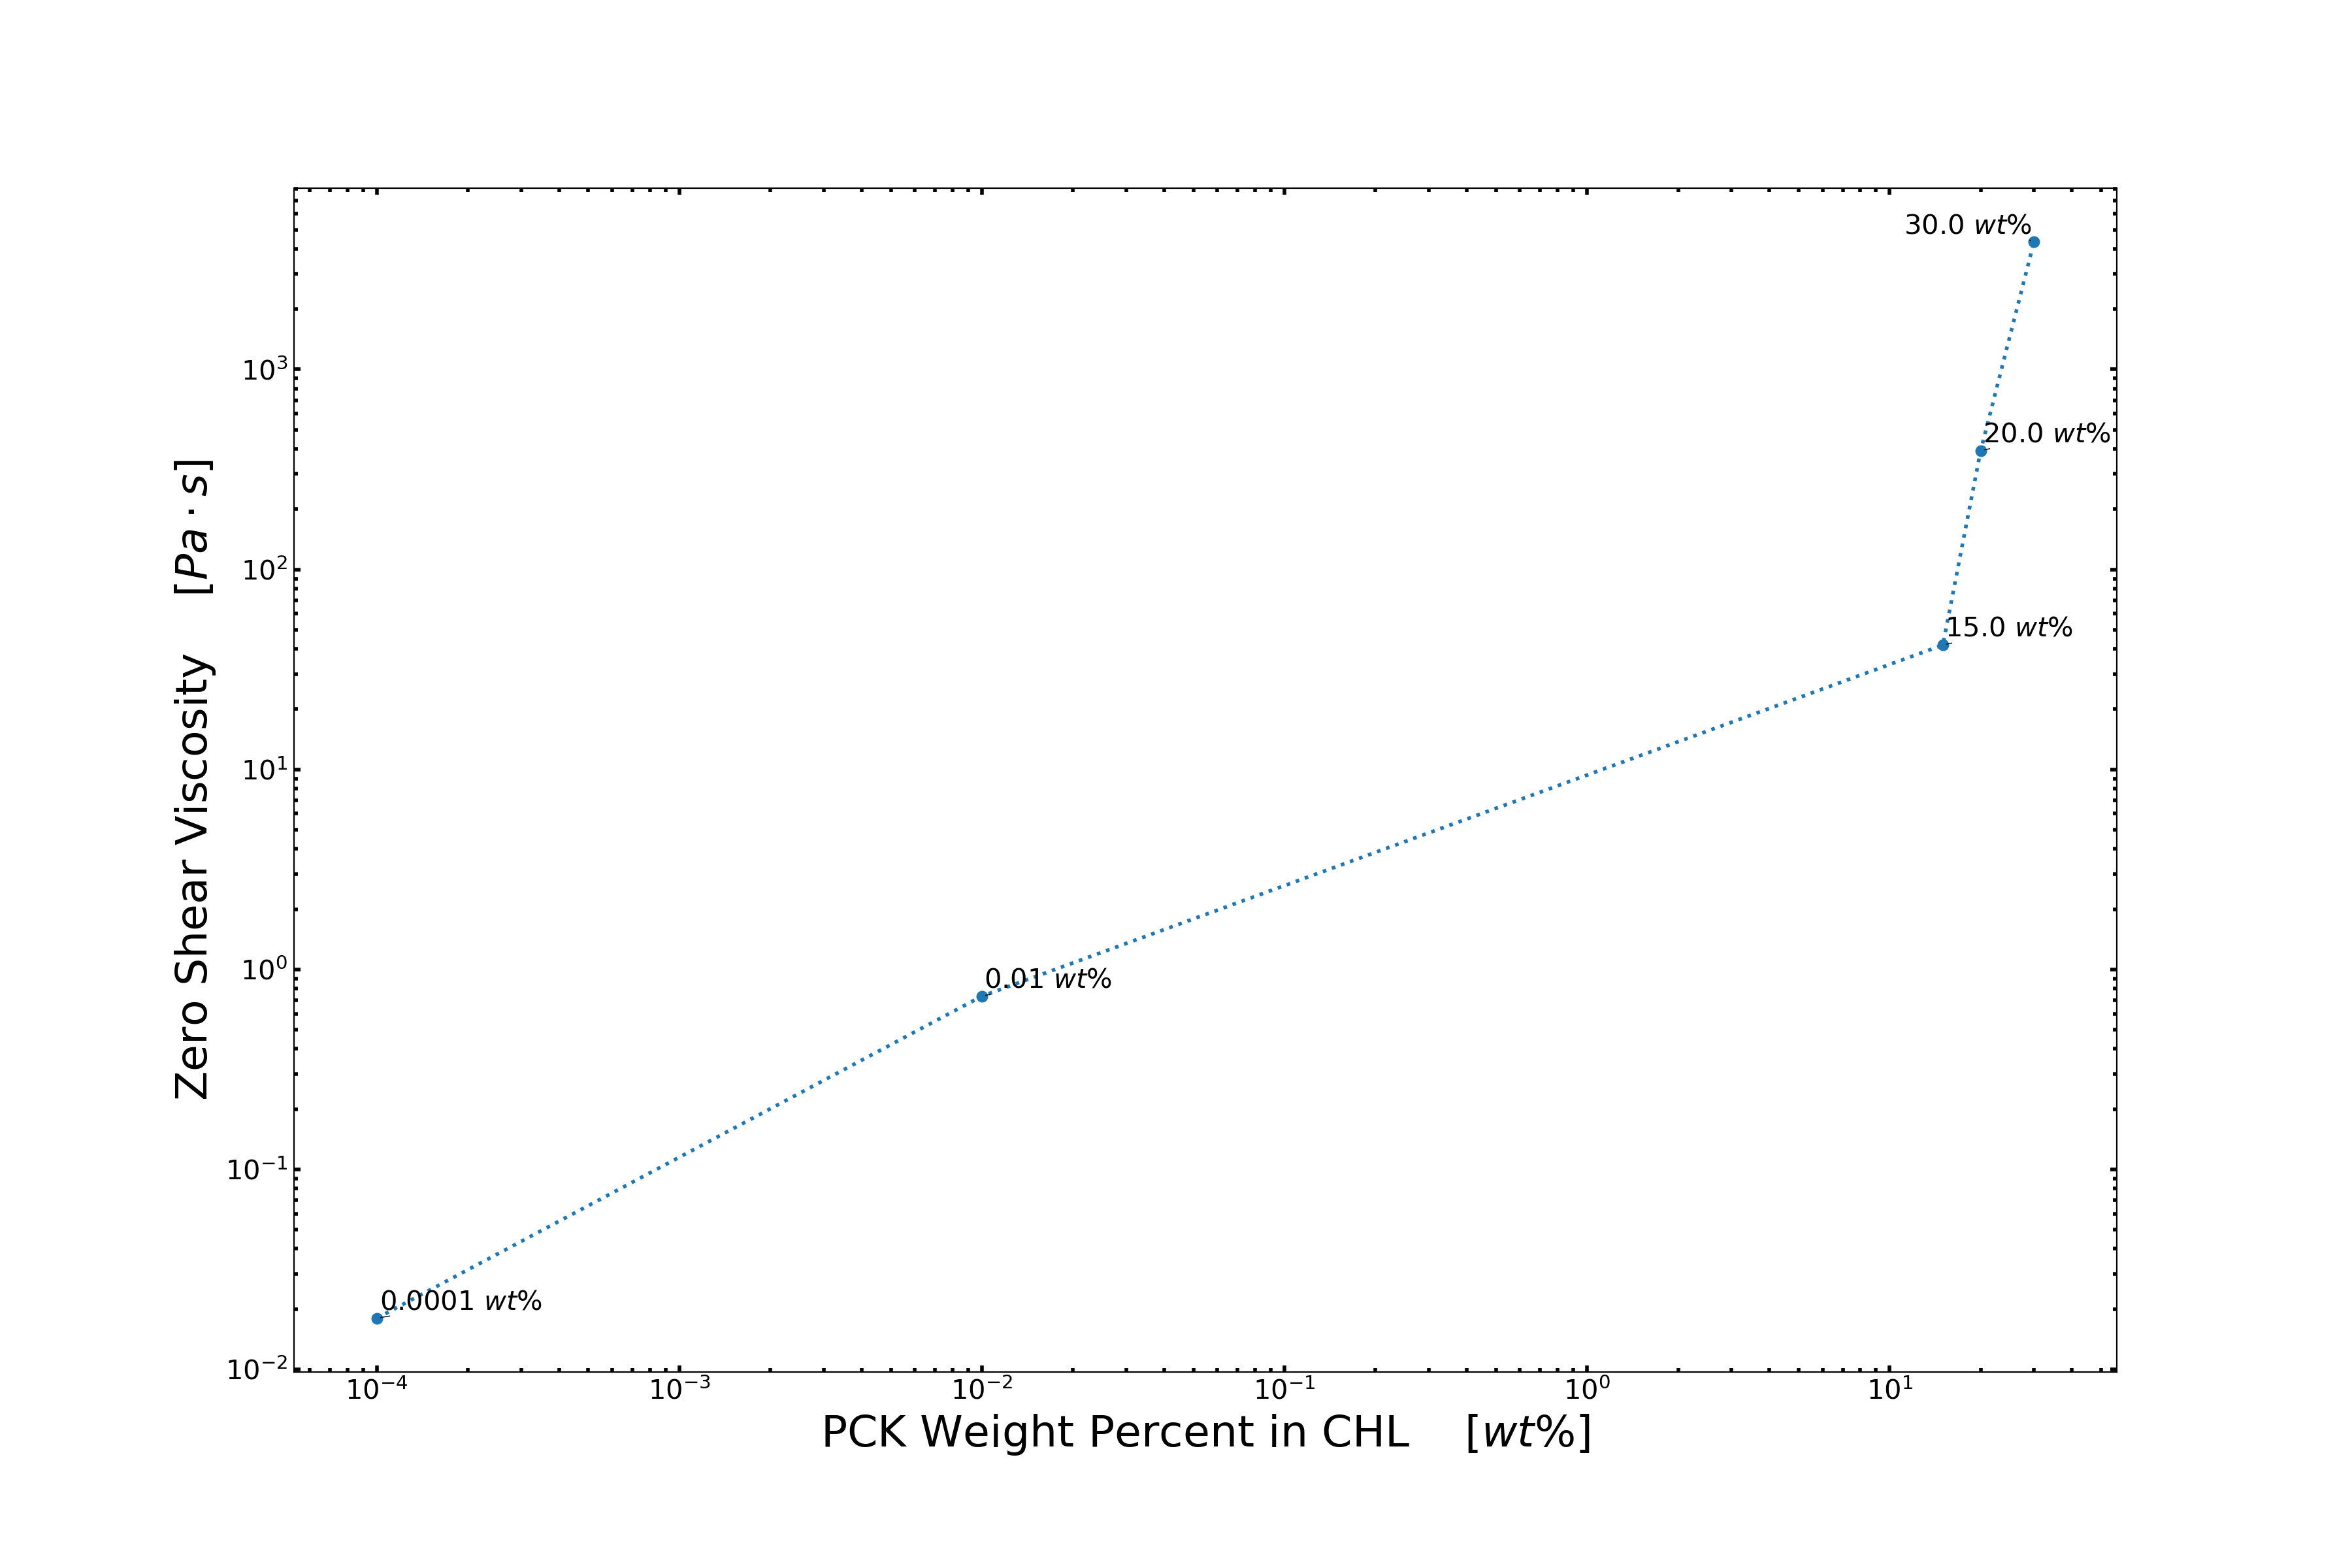
\includegraphics[width=\textwidth]{./Figures/c_vs_v_PCKinCHL.png}
\decoRule
\caption[Viscosity as a function of shear rate for Poly(9-Vinylcarbazole) (PVK) and Chloroform (CHL) solutions]{Viscosity as a function of shear rate for Poly(9-Vinylcarbazole) (PVK) and Chloroform (CHL) solutions}
\label{fig:c_vs_v_PCKinCHL}
\end{figure}

\begin{figure}[!th]
\centering
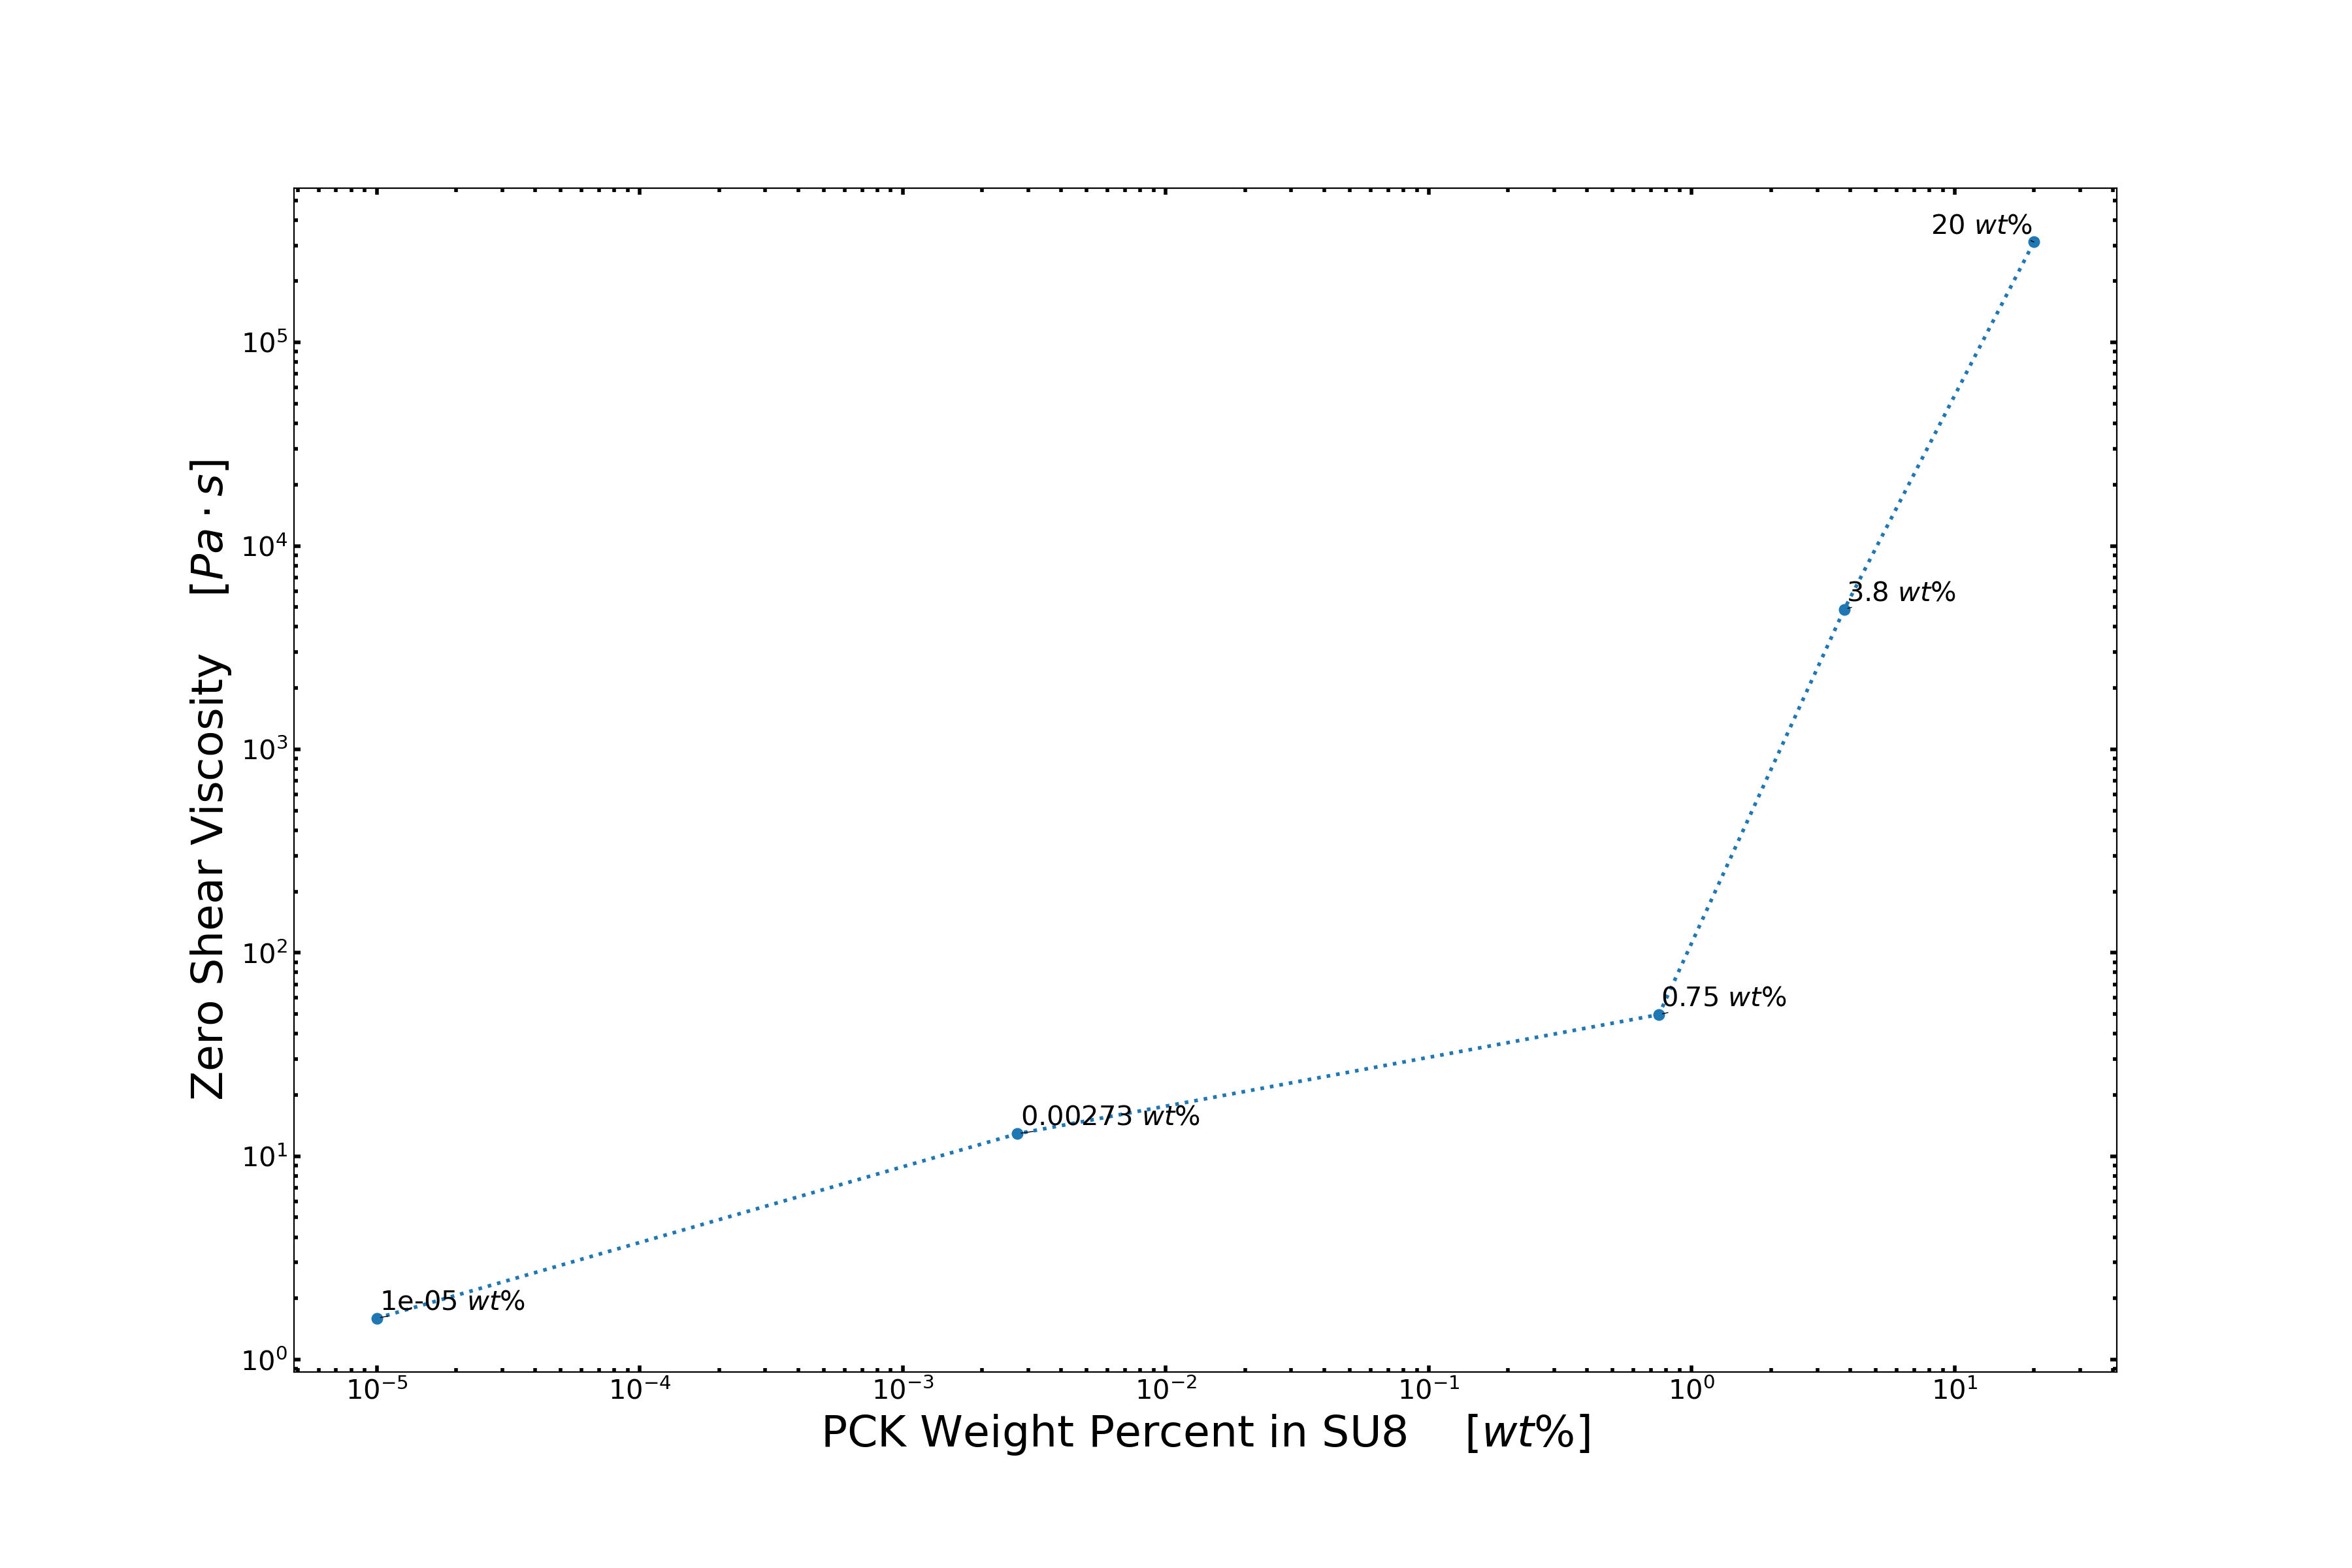
\includegraphics[width=\textwidth]{./Figures/c_vs_v_PCKinSU8.png}
\decoRule
\caption[Viscosity as a function of shear rate for Poly(9-Vinylcarbazole) (PVK) and SU-8 2002 solutions]{Viscosity as a function of shear rate for Poly(9-Vinylcarbazole) (PVK) and SU-8 2002 solutions}
\label{fig:c_vs_v_PCKinSU8}
\end{figure}